\section{01 - Intro}

\begin{definition}{What's behind the Magic?} 
    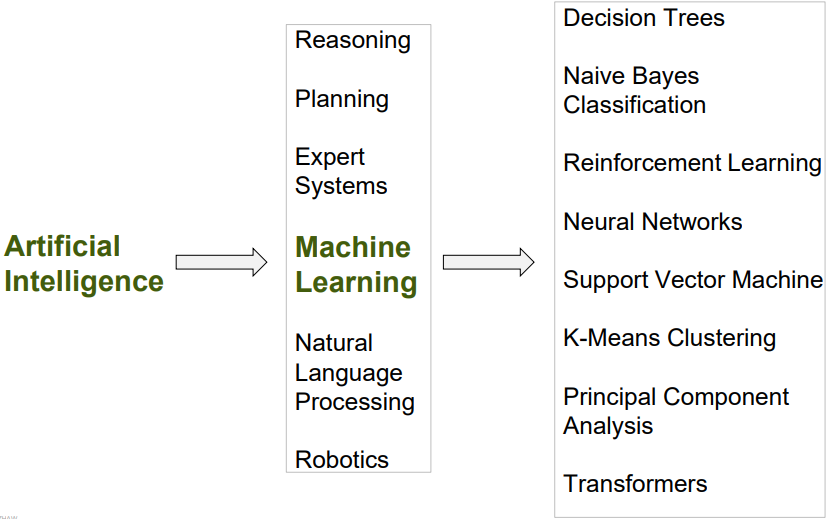
\includegraphics[width=\linewidth]{AI_magic.png}
\end{definition}

\subsection{Data Processing}

\begin{remark}
    Learning Objectives:
    \begin{itemize}
        \item Understand fundamental importance of data preprocessing
        \item Know basic algorithms for data cleaning, (near) duplicate detection and filling missing values
    \end{itemize}
\end{remark}

\subsubsection{Data}

\begin{concept}{Typical Data Driven Project}

    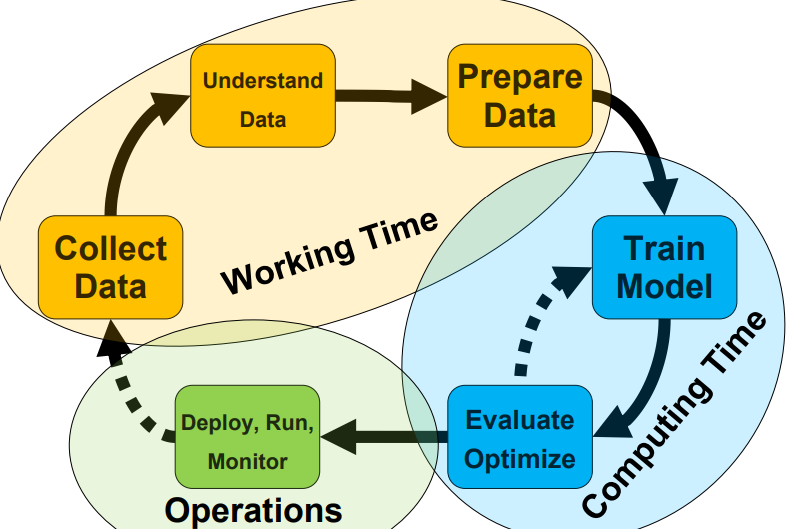
\includegraphics[width=\linewidth]{typical_data_driven_project.png}
\end{concept}

\begin{definition}{Data} has many sources, e.g.:
    \begin{itemize}
        \item sensor data
        \item survey data
        \item simulation data
        \item social media data
        \item textual data
        \item financial data
        \item multimedia data
        \item ERP systems data
    \end{itemize}
    
    Independent of the data source, each data point has a data type
\end{definition}

\begin{theorem}{Data Types}
    
    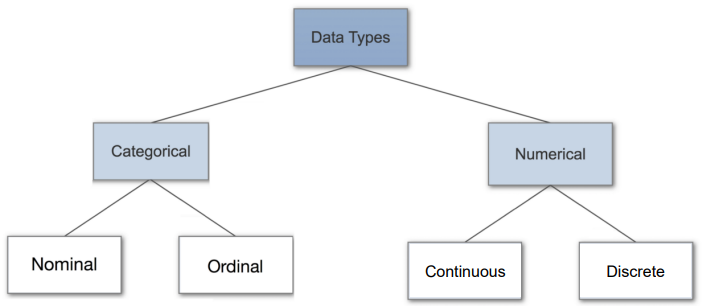
\includegraphics[width=\linewidth]{data_types.png}
\end{theorem}

\begin{corollary}{Nominal Data}
    \begin{itemize}
        \item Nominal scales are used for \textbf{labelling} variables, without any quantitative value
        \item No numerical significance
        \item Nominal data has no order
        \item Scales could simply be called labels
        \item Examples: gender, hair colour, race, marital status
    \end{itemize}
\end{corollary}

\begin{corollary}{Ordinal Data}
    \begin{itemize}
        \item Represents \textbf{discrete and ordered} units
        \item Nearly the same as nominal data, but \textbf{order matters}
        \item No distance between the different categories
        \item Examples: military rank, star rating, education level
    \end{itemize}
\end{corollary}

\begin{corollary}{Discrete Numeric Data}
    \begin{itemize}
        \item Represents items that can be \textbf{counted}
        \item Values may go from 0, 1, 2, on to infinity (making it countably infinite)
        \item Examples: number of persons in a room, number of "heads" in 60 coin flips, time elapsed in minutes
    \end{itemize}
\end{corollary}

\begin{corollary}{Continuous Numeric Data}
    \begin{itemize}
        \item Also known as \textbf{interval data}
        \item Often measurements
        \item Possible values \textbf{cannot be counted} and can only be described using intervals on the real number line
        \item Examples: temperature, weight, height, time, ...
    \end{itemize}
\end{corollary}